\newpage
\section*{Appendix A} \label{append:a}
\section*{General}
Link to the Ethics form and Participant Information Sheet:

\url{https://falmouthac-my.sharepoint.com/:f:/g/personal/to231922_falmouth_ac_uk/EiE3vOcxqLlLuU0_BN7m1NoBCja231kbqKHAxOlqX-sRfw?e=4dc65R}
\\
\\
Link to the Computing Artefact GitHub repository: 
\url{https://github.falmouth.ac.uk/TO231922/computing-artefact}
\begin{figure}[ht]
    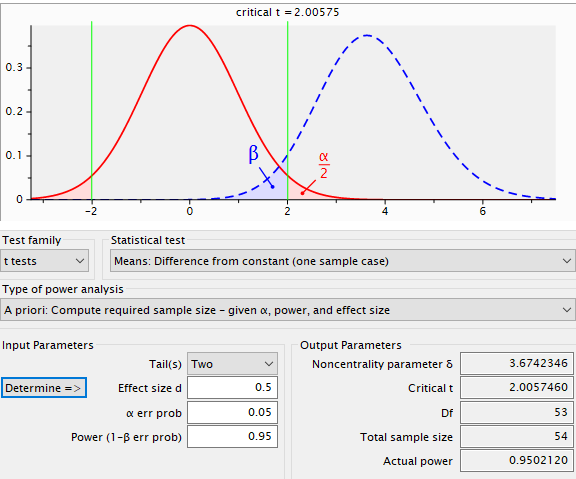
\includegraphics[width=0.48\textwidth]{./Images/gpower.png}
    \centering
    \caption{G*Power Sample Size}
    \label{gpower}
\end{figure}

\newpage
\section*{Appendix B}
\section*{Data Analysis}
\label{append:b}
\begin{lstlisting}[language=R, caption = Example R code for a Two Tailed T-Test using data from an imported CSV file]
    # Load the necessary library to read from CSV files
    library(readr)

    # Load the CSV file
    researchData <- read_csv("D:/R/ArtefactDataAnalysis/research_data.csv")

    # Perform a Two Tailed T-Test
    twoTailed <- t.test(researchData$artefactPicks , researchData$humanPicks)

    # Summarise the results
    summary(twoTailed)
\end{lstlisting}

\newpage
\section*{Appendix C}
\section*{Software Architecture}
\label{append:c}
\begin{figure}[ht]
    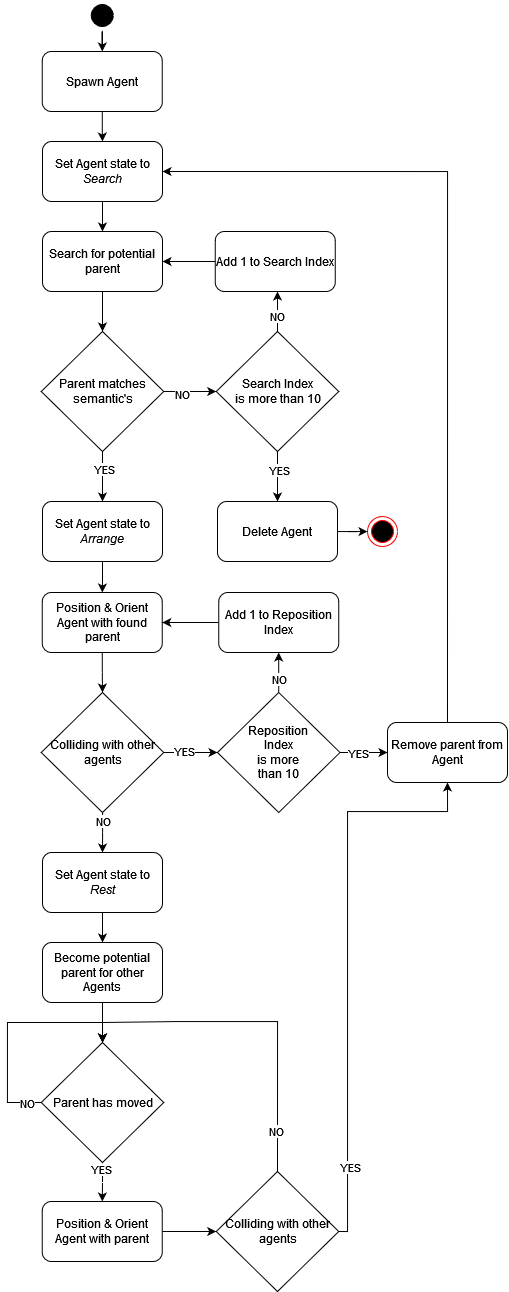
\includegraphics[width=0.45\textwidth]{./Images/AgentActivityDiagram.png}
    \centering
    \caption{Agent Behaviour represented in an Activity Diagram}
    \label{activity-diagram}
\end{figure}